\chapter{Elektrostatica: het veld en de wet van Gauss}\label{ch:b1:electrostatics-gauss}

Wrijf een ballon over een trui en hij blijft aan de muur plakken; kam droog haar en
de kam buigt een dun straaltje water af. Achter beide zit de kracht tussen
\omterm{def:b1:electrostatics-gauss:charge}{elektrische ladingen} in rust, de \omterm{thm:b1:electrostatics-gauss:coulomb}{wet van Coulomb} --- een wet van het omgekeerde kwadraat zoals
de zwaartekracht, maar $10^{36}$ keer sterker tussen twee protonen en van beide
tekens, zodat materie tot in fantastische precisie neutraal is en de
resterende effecten zijn wat wij scheikunde, materialen en bliksem noemen.
Dit hoofdstuk bouwt het begrip dat de wet hanteerbaar maakt, het
elektrische veld, laat zien hoe men een veld uit zijn symmetrieën afleest, en
leidt de ene stelling af die de velden van symmetrische verdelingen in
drie regels berekent: de \omterm{thm:b1:electrostatics-gauss:gauss}{wet van Gauss}. Haar tweelingzus voor de zwaartekracht
komt er aan het eind gratis bij.

\begin{omfigure}
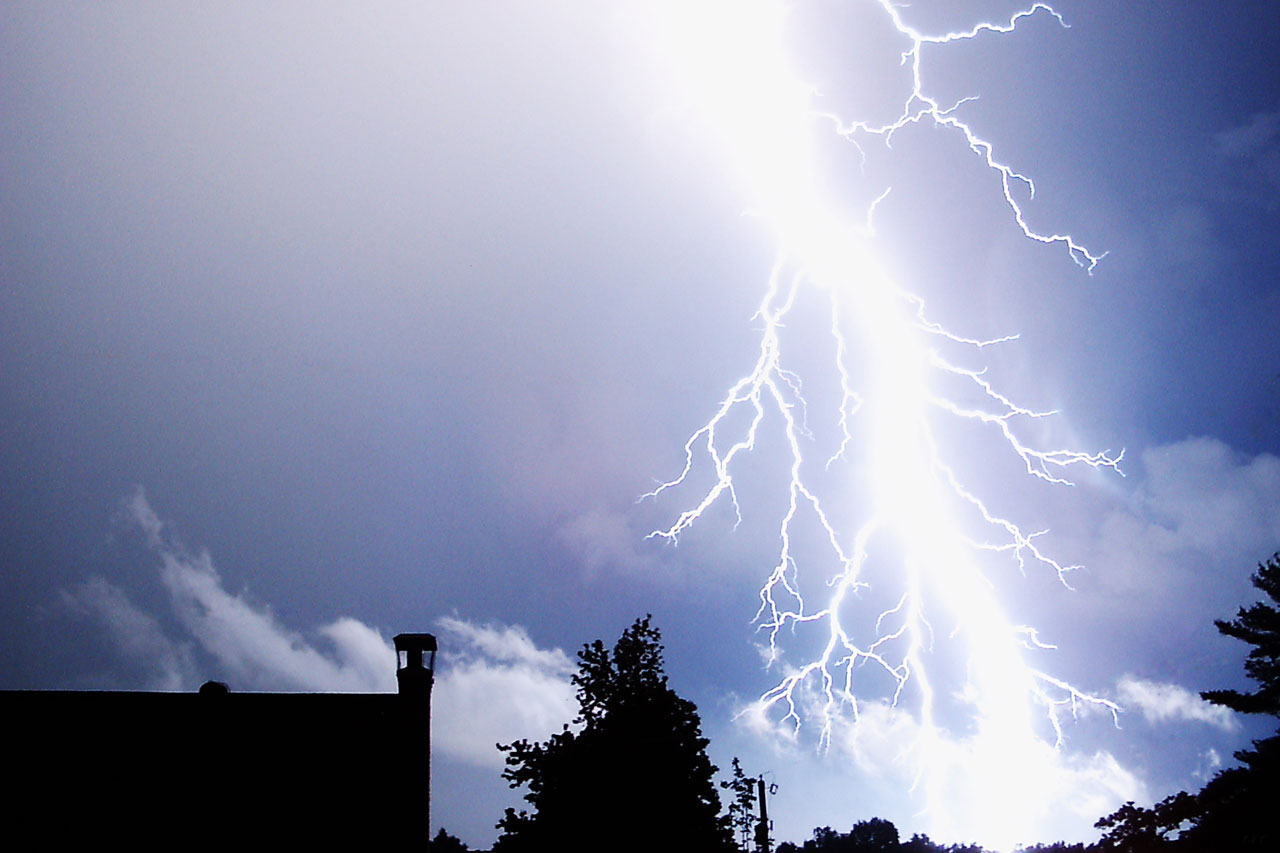
\includegraphics[width=0.50\linewidth]{images/book3/lightning-strike.jpg}

{\small Bliksem van wolk naar grond: tientallen coulomb worden in een paar ontladingen van honderd kiloampère omlaag gebracht --- de elektrische aarde van de weekendopgave.}
\end{omfigure}

\section{Ladingen en de wet van Coulomb}

\begin{definition}[Elektrische lading]\label{def:b1:electrostatics-gauss:charge}
\index{elektrische lading}\index{elementaire lading}\index{ladingsdichtheid}
\emph{Elektrische lading} $q$ (coulomb, \unit{C}) is een eigenschap van materie
met beide tekens; zij blijft behouden (de totale lading van een geïsoleerd systeem
verandert nooit) en is gekwantiseerd in eenheden van de \emph{elementaire lading}
$e = \qty{1.602e-19}{C}$ (proton $+e$, elektron $-e$). Een macroscopische
verdeling wordt beschreven door een \emph{ladingsdichtheid}: lijndichtheid $\lambda$
(\unit{C/m}), oppervlaktedichtheid $\sigma$ (\unit{C/m^2}) of ruimtedichtheid $\rho$
(\unit{C/m^3}), zodat een klein element de lading $\dd q = \lambda\,\dd l$,
$\sigma\,\dd S$ of $\rho\,\dd\tau$ draagt.
\end{definition}

\begin{theorem}[De wet van Coulomb]\label{thm:b1:electrostatics-gauss:coulomb}
\index{wet van Coulomb}\index{permittiviteit van het vacuüm}
Twee puntladingen $q_1$ in $M_1$ en $q_2$ in $M_2$ die in vacuüm in rust zijn
oefenen op elkaar de krachten
\[
\vect F_{1 \to 2} = \frac{q_1q_2}{4\pi\varepsilon_0\,r^2}\,\vect e_{12} = -\vect F_{2 \to 1},
\qquad r = M_1M_2,\quad \vect e_{12} = \frac{\vect{M_1M_2}}{r},
\]
uit, afstotend bij gelijke tekens en aantrekkend bij tegengestelde, met de
\emph{\omterm{thm:b1:electrostatics-gauss:coulomb}{permittiviteit van het vacuüm}} $\varepsilon_0 = \qty{8.854e-12}{F/m}$, dus
$1/4\pi\varepsilon_0 = \qty{8.99e9}{N.m^2/C^2}$. Krachten van meerdere ladingen tellen op
(superpositie).
\end{theorem}
\admitted

\begin{example}[Hoe sterk]\label{ex:b1:electrostatics-gauss:strong}
Twee protonen op \qty{1}{fm} afstand stoten elkaar af met $8.99 \times 10^9 \times (1.6 \times
10^{-19})^2/10^{-30} = \qty{230}{N}$ --- het gewicht van een kind, tussen twee
deeltjes van $10^{-27}$~kg; hun gravitationele aantrekking is
$10^{36}$ keer kleiner. Twee gram elektronen aan de ene kant van een kamer
en de bijbehorende protonen aan de andere zouden elkaar met $10^{25}$~N aantrekken.
Materie is neutraal omdat zij geen keus heeft: elke onbalans wordt gecorrigeerd
door krachten waartegen geen enkele structuur bestand is.
\end{example}

\section{Het elektrische veld}

\begin{definition}[Elektrostatisch veld]\label{def:b1:electrostatics-gauss:field}
\index{elektrisch veld}\index{veldlijn}
Een verdeling van ladingen in rust wekt in elk punt $M$ van de ruimte
een \emph{elektrisch veld} $\vect E(M)$ op, gedefinieerd door de kracht die het uitoefent op
een proeflading $q$ in $M$: $\vect F = q\vect E(M)$ (\unit{V/m} $=$
\unit{N/C}). Een puntlading $q_1$ in $O$ wekt
\[
\vect E(M) = \frac{q_1}{4\pi\varepsilon_0 r^2}\,\vect e_r , \qquad r = OM ,
\]
op, radiaal en naar buiten gericht voor $q_1 > 0$; een verdeling wekt de vectorsom van
de velden van haar elementen op. Een \emph{veldlijn} is een kromme die in elk
punt raakt aan $\vect E$ en er langs georiënteerd is.
\end{definition}

\begin{proposition}[Een veldkaart lezen]\label{prop:b1:electrostatics-gauss:lines}
\omterm{def:b1:electrostatics-gauss:field}{Veldlijnen} vertrekken bij positieve ladingen en eindigen op negatieve (of in
het oneindige); zij kruisen elkaar nooit (het veld is eenduidig), en zij
dringen samen waar het veld sterk is. Zijn er twee ladingen aanwezig, dan is het
aantal lijnen dat men bij elk tekent evenredig met haar lading.
\end{proposition}

\begin{omfigure}
\begin{tikzpicture}[font=\small, x=1cm, y=1cm, >=Stealth]
  % dipole: arcs through (-1,0) and (1,0), centre (0,c)
  \begin{scope}[scale=1.4]
    \foreach \c in {0.1, 0.55, 1.6} {
      \draw[omDef, thick, postaction={decorate, decoration={markings, mark=at position 0.5 with {\arrow{>}}}}]
        let \n1 = {sqrt(1+\c*\c)} in
        (-1,0) arc[start angle={180+atan2(\c,1)}, end angle={360-atan2(\c,1)}, radius=\n1 cm];
      \draw[omDef, thick, postaction={decorate, decoration={markings, mark=at position 0.5 with {\arrow{>}}}}]
        let \n1 = {sqrt(1+\c*\c)} in
        (-1,0) arc[start angle={180-atan2(\c,1)}, end angle={atan2(\c,1)}, radius=\n1 cm];
    }
    \draw[omDef, thick, postaction={decorate, decoration={markings, mark=at position 0.5 with {\arrow{>}}}}] (-1,0) -- (1,0);
    \draw[omDef, thick, postaction={decorate, decoration={markings, mark=at position 0.6 with {\arrow{>}}}}] (-2.6,0) -- (-1,0);
    \draw[omDef, thick, postaction={decorate, decoration={markings, mark=at position 0.4 with {\arrow{>}}}}] (1,0) -- (2.6,0);
    \fill[omThm] (-1,0) circle (3pt) node[below left] {$+q$};
    \fill[omDef] (1,0) circle (3pt) node[below right] {$-q$};
  \end{scope}
  % two like charges
  \begin{scope}[xshift=7.9cm, fl/.style={omThm, thick, postaction={decorate, decoration={markings, mark=at position 0.55 with {\arrow{>}}}}}]
    \foreach \s in {1,-1} {
      % left charge at (-1,0), right charge at (1,0); \s mirrors up/down
      \draw[fl] (-1,0) -- (-3.4,0);
      \draw[fl] (1,0) -- (3.4,0);
      \draw[fl] (-1,0) .. controls (-2.2,{1.2*\s}) .. (-3.2,{2.0*\s});
      \draw[fl] (1,0) .. controls (2.2,{1.2*\s}) .. (3.2,{2.0*\s});
      \draw[fl] (-1,0) .. controls (-1.1,{1.3*\s}) .. (-1.6,{2.9*\s});
      \draw[fl] (1,0) .. controls (1.1,{1.3*\s}) .. (1.6,{2.9*\s});
      \draw[fl] (-1,0) .. controls (-0.2,{0.7*\s}) and (-0.1,{1.6*\s}) .. (-0.3,{2.9*\s});
      \draw[fl] (1,0) .. controls (0.2,{0.7*\s}) and (0.1,{1.6*\s}) .. (0.3,{2.9*\s});
    }
    \draw[fl] (-1,0) -- (-0.08,0);
    \draw[fl] (1,0) -- (0.08,0);
    \fill[omThm] (-1,0) circle (3pt) node[below left] {$+q$};
    \fill[omThm] (1,0) circle (3pt) node[below right] {$+q$};
    \fill (0,0) circle (1.2pt) node[below, font=\footnotesize, yshift=-2pt] {$\vect E = \vect 0$};
  \end{scope}
\end{tikzpicture}

{\small \omterm{def:b1:electrostatics-gauss:field}{Veldlijnen} van twee tegengestelde ladingen (links) en van twee gelijke
positieve ladingen (rechts). Lijnen beginnen op $+$ en eindigen op $-$ of in
het oneindige; rechts stoten zij elkaar af en verdwijnt het veld in
het middelpunt, waar geen lijn passeert.}
\end{omfigure}

\begin{example}[Ring en segment door rechtstreeks sommeren]\label{ex:b1:electrostatics-gauss:ring}
Op de as van een ring met straal $R$ die $Q$ gelijkmatig draagt, op afstand
$z$ van het middelpunt, levert elk element $\dd q$ een bijdrage $\dd q/4\pi\varepsilon_0(R^2 +
z^2)$ langs de lijn die het met $M$ verbindt; de componenten loodrecht
op de as vallen paarsgewijs weg en de axiale tellen op met de factor
$z/\sqrt{R^2 + z^2}$:
\[
E_z = \frac{Qz}{4\pi\varepsilon_0(R^2 + z^2)^{3/2}} ,
\]
nul in het middelpunt, maximaal bij $z = R/\sqrt2$, en $Q/4\pi\varepsilon_0z^2$ ver
weg. Een gelijkmatig geladen schijf is een stapel ringen (\cref{pb:b1:electrostatics-gauss:1}).
Rechtstreeks sommeren werkt telkens wanneer de meetkunde de integraal toelaat; de
rest van dit hoofdstuk gaat erover hem te vermijden.
\end{example}

\section{Symmetrieën en invarianties}

\begin{proposition}[Symmetriebeginsel]\label{prop:b1:electrostatics-gauss:symmetry}
\index{symmetrie (van een veld)}\index{symmetrievlak}\index{antisymmetrievlak}
Het veld heeft de symmetrieën van zijn bronnen. Is een vlak $\Pi$ een
\emph{\omterm{prop:b1:electrostatics-gauss:symmetry}{symmetrievlak}} van de ladingsverdeling (het spiegelbeeld
van de verdeling is zijzelf), dan ligt het veld in elk punt van $\Pi$
\emph{in} $\Pi$; is $\Pi$ een \emph{\omterm{prop:b1:electrostatics-gauss:symmetry}{antisymmetrievlak}}
(het spiegelbeeld is de verdeling met alle ladingen omgekeerd), dan staat het
veld in de punten van $\Pi$ \emph{loodrecht} op $\Pi$. Is de
verdeling invariant onder een translatie of een rotatie, dan is het veld dat ook:
zijn componenten hangen niet van de bijbehorende coördinaat af.
\end{proposition}

\begin{proof}
$\vect E$ is een som van termen $\dd q\,\vect e/4\pi\varepsilon_0r^2$; het spiegelbeeld
van de som is de som van de spiegelbeelden, en het beeld van het veld
van een verdeling is het veld van de gespiegelde verdeling (een vector die
uit posities en ladingen is opgebouwd transformeert zoals de posities). Op een
\omterm{prop:b1:electrostatics-gauss:symmetry}{symmetrievlak} is het veld gelijk aan zijn eigen spiegelbeeld en ligt het dus in het
vlak; op een \omterm{prop:b1:electrostatics-gauss:symmetry}{antisymmetrievlak} is het gelijk aan het tegengestelde van zijn beeld en
staat het er dus loodrecht op. Voor invariantie geldt hetzelfde argument met een
translatie of rotatie.
\end{proof}

\begin{method}[De vorm van een veld bepalen vóór men het berekent]\label{meth:b1:electrostatics-gauss:symmetry}
Voor het punt $M$ waar men het veld wil hebben: (1) som de symmetrievlakken
van de bronnen op die $M$ bevatten --- het veld ligt op hun
snijlijn; twee zulke vlakken leggen de richting vast. (2) Som de
invarianties op --- die zeggen van welke coördinaten $\vect E$ afhangt. Zo geeft een
gelijkmatig geladen oneindige draad $\vect E = E(r)\,\vect e_r$ in
\omterm{def:b1:point-kinematics:cylindrical}{cilindercoördinaten}, een bol $\vect E = E(r)\,\vect e_r$ in \omterm{def:b1:point-kinematics:spherical}{bolcoördinaten},
en een oneindig vlak $\vect E = E(z)\,\vect e_z$ met $E(-z) = -E(z)$.
Pas daarna rekent men.
\end{method}

\begin{omfigure}
\begin{tikzpicture}[font=\small, x=1cm, y=1cm, >=Stealth]
  % sphere
  \begin{scope}
    \draw[omDef, fill=omDef!15] (0,0) circle (0.9);
    \draw[dashed] (0,0) circle (1.8);
    \foreach \a in {0,45,...,315} \draw[omThm, thick, ->] (\a:1.8) -- ++(\a:0.6);
    \node[font=\footnotesize] at (0,-2.75) {$\vect E = E(r)\,\vect e_r$};
    \node[font=\footnotesize, omDef] at (0,0) {$Q$};
  \end{scope}
  % cylinder / wire
  \begin{scope}[xshift=5.2cm]
    \draw[omDef, very thick] (0,-2.2) -- (0,2.2) node[above, font=\footnotesize] {$\lambda$};
    \draw[dashed] (-1.1,-1.6) rectangle (1.1,1.6);
    \draw[dashed] (0,1.6) ellipse (1.1 and 0.28);
    \draw[dashed] (0,-1.6) ellipse (1.1 and 0.28);
    \foreach \y in {-1.0,-0.3,0.4,1.1} {\draw[omThm, thick, ->] (1.1,\y) -- ++(0.6,0); \draw[omThm, thick, ->] (-1.1,\y) -- ++(-0.6,0);}
    \node[font=\footnotesize] at (0,-2.75) {$\vect E = E(r)\,\vect e_r$ (cilindrisch)};
  \end{scope}
  % plane
  \begin{scope}[xshift=10.4cm]
    \draw[omDef, fill=omDef!25] (-1.8,-0.25) -- (1.8,-0.25) -- (2.2,0.25) -- (-1.4,0.25) -- cycle;
    \node[omDef, font=\footnotesize] at (1.9,-0.45) {$\sigma$};
    \draw[dashed] (-0.5,-1.4) rectangle (0.5,1.4);
    \foreach \x in {-1.2,0,1.2} {\draw[omThm, thick, ->] (\x,0.35) -- ++(0,0.9); \draw[omThm, thick, ->] (\x,-0.35) -- ++(0,-0.9);}
    \node[font=\footnotesize] at (0,-2.75) {$\vect E = E(z)\,\vect e_z$, oneven in $z$};
  \end{scope}
\end{tikzpicture}

{\small De drie symmetrische verdelingen van dit hoofdstuk en de
gaussoppervlakken (gestippeld) die erbij passen: een concentrische bol, een
coaxiale cilinder, een doosje dat het vlak omvat. Op elk staat het veld
óf loodrecht met overal dezelfde grootte, óf raakt het.}
\end{omfigure}

\section{Flux en de wet van Gauss}

\begin{definition}[Flux van het veld]\label{def:b1:electrostatics-gauss:flux}
\index{flux van het elektrische veld}
Verdeel een oppervlak $S$ in kleine elementen met oppervlakte $\dd S$, elk met een
eenheidsnormaal $\vect n$ (bij een gesloten oppervlak de buitennormaal). De
\emph{flux} van $\vect E$ door $S$ is de som
\[
\Phi = \sum \vect E\cdot\vect n\,\dd S = \sum E_n\,\dd S \qquad (\unit{V.m}):
\]
de normale component van het veld gewogen met de oppervlakte --- het ``aantal
\omterm{def:b1:electrostatics-gauss:field}{veldlijnen}'' dat $S$ kruist, positief geteld wanneer zij langs
$\vect n$ kruisen.
\end{definition}

\begin{theorem}[De wet van Gauss]\label{thm:b1:electrostatics-gauss:gauss}
\index{wet van Gauss}
De \omterm{def:b1:electrostatics-gauss:flux}{flux} van het elektrostatische veld door een willekeurig gesloten oppervlak $S$
is gelijk aan de totale lading die $S$ omsluit, gedeeld door $\varepsilon_0$:
\[
\Phi_{\text{uit}} = \frac{Q_{\text{binnen}}}{\varepsilon_0} .
\]
Ladingen buiten $S$ dragen niets aan de \omterm{def:b1:electrostatics-gauss:flux}{flux} bij (hun lijnen gaan erin
en komen er weer uit).
\end{theorem}

\begin{proof}
Voor een puntlading $q$ in het middelpunt van een bol met straal $r$ is
$\vect E$ radiaal en overal op de bol even groot, $q/4\pi\varepsilon_0r^2$,
zodat $\Phi = E \times 4\pi r^2 = q/\varepsilon_0$ --- onafhankelijk van $r$,
omdat het veld precies zo als $1/r^2$ afneemt als de oppervlakte groeit. Dat
hetzelfde geldt voor elk gesloten oppervlak om $q$ (de \omterm{def:b1:electrostatics-gauss:flux}{flux} door een
oppervlakte-element hangt alleen af van de ruimtehoek waaronder het vanuit $q$ wordt gezien),
dat een lading erbuiten nul geeft (zij spant elke ruimtehoek twee keer op,
met tegengesteld teken), en dat de \omterm{def:b1:electrostatics-gauss:flux}{fluxen} van meerdere ladingen optellen, wordt
hier aangenomen; het volledige bewijs staat in het volume van jaar 2.
\end{proof}

\begin{method}[De wet van Gauss gebruiken]\label{meth:b1:electrostatics-gauss:gauss}
(1) Schrijf uit de symmetrieën de vorm van $\vect E$ op (richting en de
variabele waarvan het afhangt). (2) Kies een gesloten \emph{gaussoppervlak}
door het punt $M$ waarop $\vect E$ overal óf loodrecht staat met
dezelfde grootte $E(M)$, óf raakt: de \omterm{def:b1:electrostatics-gauss:flux}{flux} is dan $E(M)$ maal de
oppervlakte van het loodrechte deel. (3) Tel de lading erbinnen. (4) Los op naar
$E(M)$. Het werkt voor bollen, oneindige cilinders en oneindige vlakken
--- en zonder verder gereedschap voor niets anders.
\end{method}

\begin{proposition}[De drie klassieke velden]\label{prop:b1:electrostatics-gauss:three}
\index{veld van een geladen bol}\index{veld van een geladen draad}\index{veld van een geladen vlak}
\begin{enumerate}
  \item Bol met straal $R$ en lading $Q$ gelijkmatig over zijn
        volume verdeeld: $E(r) = \dfrac{Q}{4\pi\varepsilon_0r^2}$ erbuiten ($r > R$) ---
        alsof alle lading in het middelpunt zat --- en $E(r) =
        \dfrac{Qr}{4\pi\varepsilon_0R^3}$ erbinnen, lineair groeiend vanaf nul;
        continu in $r = R$. Zit de lading alleen op het oppervlak,
        dan is het veld binnenin nul.
  \item Oneindige draad met lijnlading $\lambda$: $E(r) =
        \dfrac{\lambda}{2\pi\varepsilon_0 r}$, radiaal.
  \item Oneindig vlak met oppervlaktelading $\sigma$: $E = \dfrac{\sigma}{2\varepsilon_0}$
        aan weerszijden, loodrecht op het vlak, ervan af gericht bij
        $\sigma > 0$, \emph{onafhankelijk van de afstand}. Over het vlak heen
        springt de normale component met $\sigma/\varepsilon_0$.
\end{enumerate}
\end{proposition}

\begin{proof}
(1) Bol met straal $r$: \omterm{def:b1:electrostatics-gauss:flux}{flux} $4\pi r^2E(r)$; lading erbinnen $Q$ als
$r > R$, $Q(r/R)^3$ als $r < R$. (2) Cilinder met straal $r$ en lengte $h$:
\omterm{def:b1:electrostatics-gauss:flux}{flux} door het zijoppervlak $2\pi rh\,E(r)$, geen door de eindvlakken
(veld rakend); lading $\lambda h$. (3) Doosje met doorsnede $S$
dat het vlak omvat: \omterm{def:b1:electrostatics-gauss:flux}{flux} $2SE$ door de twee eindvlakken (het veld is oneven
in $z$, zodat beide positief tellen), geen door de zijkant; lading
$\sigma S$.
\end{proof}

\begin{omfigure}
\begin{tikzpicture}
\begin{axis}[omaxis, axis x line=bottom, axis y line=left, width=10cm, height=5.6cm,
    xlabel={$r/R$}, ylabel={$E$ (in eenheden van $Q/4\pi\varepsilon_0R^2$)},
    xlabel style={at={(axis description cs:0.5,-0.1)}, anchor=north},
    xmin=0, xmax=4, ymin=0, ymax=1.3, xtick={1,2,3}, ytick={0.5,1}, samples=80]
  \addplot[omDef, very thick, domain=0:1] {x} node[pos=0.85, above left, font=\footnotesize] {volume: $\propto r$};
  \addplot[omDef, very thick, domain=1:4] {1/x^2} node[pos=0.35, above right, font=\footnotesize] {$\propto 1/r^2$};
  \addplot[omThm, thick, dashed] coordinates {(0,0) (1,0)};
  \addplot[omThm, thick, dashed] coordinates {(1,0) (1,1)};
  \node[omThm, font=\footnotesize, anchor=west] at (axis cs:1.08,0.08) {oppervlak: $0$ binnenin};
\end{axis}
\end{tikzpicture}

{\small Het \omterm{prop:b1:electrostatics-gauss:three}{veld van een geladen bol} tegen de afstand tot zijn middelpunt:
lineair binnenin en als $1/r^2$ erbuiten wanneer de lading het volume vult
(doorgetrokken); nul binnenin en hetzelfde erbuiten wanneer zij op het oppervlak zit
(gestippeld). Buiten onderscheidt niets de bol van een puntlading
in haar middelpunt.}
\end{omfigure}

\begin{example}[Twee vlakken: de vlakke condensator]\label{ex:b1:electrostatics-gauss:twoplanes}
\index{vlakke condensator!veld}
Twee evenwijdige vlakken die $+\sigma$ en $-\sigma$ dragen: elk wekt
$\sigma/2\varepsilon_0$ op, van zich af gericht (naar zich toe bij het negatieve).
Tussen de vlakken tellen de twee velden op tot $\sigma/\varepsilon_0$, gericht van
$+$ naar $-$; erbuiten heffen zij elkaar op. Met $\sigma = \qty{1}{\micro C/m^2}$ is $E =
10^{-6}/8.85 \times 10^{-12} = \qty{1.1e5}{V/m}$ ertussen en nul erbuiten: het
veld van een geladen condensator zit opgesloten in zijn spleet
(\cref{ch:b1:potential-capacitors}).
\end{example}

\begin{omfigure}
\begin{tikzpicture}[font=\small, x=1cm, y=1cm, >=Stealth]
  \draw[omThm, very thick] (-0.8,-2) -- (-0.8,2) node[above] {$+\sigma$};
  \draw[omDef, very thick] (0.8,-2) -- (0.8,2) node[above] {$-\sigma$};
  % field of + plane (red), of - plane (blue), resultant (black)
  \foreach \y in {-1.4,-0.7,0,0.7,1.4} {
    \draw[omThm, ->] (-0.8,\y) -- ++(0.55,0);
    \draw[omThm, ->] (-0.8,\y) -- ++(-0.55,0);
    \draw[omDef, ->] (0.8,\y) -- ++(-0.55,0);
    \draw[omDef, ->] (0.8,\y) -- ++(0.55,0);
  }
  \node[omThm, font=\footnotesize, anchor=east] at (-1.0,-2.4) {$+\sigma$ alleen: $\sigma/2\varepsilon_0$};
  \node[omDef, font=\footnotesize, anchor=west] at (1.0,-2.4) {$-\sigma$ alleen: $\sigma/2\varepsilon_0$};
  \begin{scope}[xshift=7.2cm]
    \draw[omThm, very thick] (-0.8,-2) -- (-0.8,2) node[above] {$+\sigma$};
    \draw[omDef, very thick] (0.8,-2) -- (0.8,2) node[above] {$-\sigma$};
    \foreach \y in {-1.4,-0.7,0,0.7,1.4} \draw[black, very thick, ->] (-0.75,\y) -- (0.7,\y);
    \node[font=\footnotesize] at (0,-2.4) {totaal: $\sigma/\varepsilon_0$ ertussen, $0$ erbuiten};
  \end{scope}
\end{tikzpicture}

{\small Superpositie voor twee tegengestelde vlakken. Links: de homogene velden
van elk vlak afzonderlijk (rood vanaf het positieve, blauw naar het negatieve
toe). Rechts: hun som, $\sigma/\varepsilon_0$ in de spleet en nul elders.}
\end{omfigure}

\section{De analogie met de zwaartekracht}

\begin{proposition}[De wet van Gauss voor de zwaartekracht]\label{prop:b1:electrostatics-gauss:gravity}
\index{wet van Gauss!voor de gravitatie}\index{zwaartekrachtveld}
De wet van Newton $\vect F = -Gm_1m_2\,\vect e_{12}/r^2$ heeft de vorm van die
van Coulomb met $q \to m$ en $1/4\pi\varepsilon_0 \to -G$. Het \omterm{prop:b1:newton-dynamics:weight}{zwaartekrachtveld}
$\vect g$ (kracht per massa-eenheid) gehoorzaamt dus aan dezelfde symmetrieregels
en aan
\[
\Phi_{\text{uit}}(\vect g) = -4\pi G\,M_{\text{binnen}} .
\]
In het bijzonder trekt een bolsymmetrisch lichaam punten erbuiten aan alsof
zijn massa in zijn middelpunt zat, en is het veld binnen een homogene bol
met straal $R$ en massa $M$ gelijk aan $g(r) = GMr/R^3$, lineair in $r$.
\end{proposition}

\begin{proof}
Vervang $Q/\varepsilon_0$ door $-4\pi GM$ in het bewijs van
\cref{prop:b1:electrostatics-gauss:three}; het minteken zegt dat de \omterm{def:b1:electrostatics-gauss:flux}{flux}
naar binnen gaat (de zwaartekracht trekt aan).
\end{proof}

\begin{example}[Binnen in de aarde]\label{ex:b1:electrostatics-gauss:earth}
Voor een homogene aarde zou $g$ lineair dalen van \qty{9.8}{m/s^2} aan het
oppervlak tot nul in het middelpunt; een steen die in een tunnel dwars door
de planeet valt zou harmonisch trillen met periode $2\pi\sqrt{R/g} =
\qty{84}{min}$ --- de periode van een scherend cirkelende satelliet. De echte aarde heeft
een dichte kern, en $g$ \emph{stijgt} in werkelijkheid tot \qty{10.7}{m/s^2} op de
grens kern--mantel voordat het daalt (\cref{pb:b1:electrostatics-gauss:1}).
Newton had de schaalstelling nodig om zijn wet op planeten toe te passen; de \omterm{thm:b1:electrostatics-gauss:gauss}{wet
van Gauss} geeft haar in één regel.
\end{example}

\section{Oefeningen}

\begin{exercise}[$\star$]\label{exo:b1:electrostatics-gauss:1}
Elektrische en gravitationele kracht tussen twee protonen op
\qty{2.0}{fm} afstand; hun verhouding. Waarom houden kernen dan toch samen?
\end{exercise}

\begin{exercise}[$\star$]\label{exo:b1:electrostatics-gauss:2}
Veld op \qty{1.0}{m} van een puntlading van \qty{1.0}{\micro C}. Het aardoppervlak
draagt een veld van \qty{100}{V/m} dat naar beneden wijst: teken en waarde van
de lading van de aarde, opgevat als een bol met straal \qty{6370}{km}.
\end{exercise}

\begin{exercise}[$\star$]\label{exo:b1:electrostatics-gauss:3}
Twee ladingen $+q$ in $x = \pm a$ op de $x$-as. Veld op de $x$-as
voor $|x| > a$ en op de $y$-as; toon aan dat op de $y$-as $E_y$
maximaal is in $y = a/\sqrt2$. Schets de lijnen bij de oorsprong.
\end{exercise}

\begin{exercise}[$\star$]\label{exo:b1:electrostatics-gauss:4}
Ladingen $+2q$ in $x = 0$ en $-q$ in $x = a$. Waar op de $x$-as verdwijnt
het veld? Hoeveel \omterm{def:b1:electrostatics-gauss:field}{veldlijnen} vertrekken bij $+2q$ voor elke lijn
die bij $-q$ aankomt, en waar gaan de overige heen?
\end{exercise}

\begin{exercise}[$\star\star$]\label{exo:b1:electrostatics-gauss:5}
Een schijf met straal $R$ draagt $\sigma$ gelijkmatig. Toon met het resultaat voor de ring
aan dat op haar as $E_z = \dfrac{\sigma}{2\varepsilon_0}\Bigl(1 - \dfrac{z}{\sqrt{z^2 +
R^2}}\Bigr)$ voor $z > 0$; controleer de twee limieten $z \ll R$ en $z \gg R$.
\end{exercise}

\begin{exercise}[$\star\star$]\label{exo:b1:electrostatics-gauss:6}
Een goudkern ($Z = 79$, $R = \qty{7.0}{fm}$) als een gelijkmatig geladen
bol: veld aan het oppervlak, in $R/2$, op \qty{1}{pm}. Vergelijk met het
doorslagveld van lucht, \qty{3e6}{V/m}.
\end{exercise}

\begin{exercise}[$\star\star$]\label{exo:b1:electrostatics-gauss:7}
Veld van een oneindige draad met de \omterm{thm:b1:electrostatics-gauss:gauss}{wet van Gauss}. Een hoogspanningsgeleider met
straal \qty{1.0}{cm}: lijnlading waarbij het veld aan zijn oppervlak
de doorslagwaarde \qty{3e6}{V/m} bereikt (het inzetten van corona). Veld op
\qty{5}{m} dan.
\end{exercise}

\begin{exercise}[$\star\star$]\label{exo:b1:electrostatics-gauss:8}
Twee evenwijdige platen met oppervlakte \qty{1.0}{m^2} dragen $\pm\qty{1.0}{\micro C}$.
Veld ertussen; kracht op één plaat (het veld dat erop werkt is alleen dat
van de andere plaat --- waarom?); druk op de platen.
\end{exercise}

\begin{exercise}[$\star\star$]\label{exo:b1:electrostatics-gauss:9}
Coaxkabel: binnengeleider met straal $a$ en $+\lambda$, buitenmantel
met straal $b$ en $-\lambda$. Veld in de drie gebieden met
de \omterm{thm:b1:electrostatics-gauss:gauss}{wet van Gauss}. $a = \qty{0.5}{mm}$, $b = \qty{2.5}{mm}$, $\lambda = \qty{10}{nC/m}$:
veld aan het oppervlak van de binnengeleider.
\end{exercise}

\begin{exercise}[$\star\star\star$]\label{exo:b1:electrostatics-gauss:10}
Een dikke bolschil $R_1 < r < R_2$ draagt $Q$ gelijkmatig in haar
volume. Veld in de drie gebieden; controleer de continuïteit in $R_1$ en
$R_2$; waar is het maximaal? Schets $E(r)$. Een positieve lading die
in de holte wordt gelegd: welke kracht voelt zij?
\end{exercise}

\begin{exercise}[$\star\star\star$]\label{exo:b1:electrostatics-gauss:11}
\emph{Zwaartekracht binnen in de aarde.} Kern: straal \qty{3480}{km}, dichtheid
\qty{11000}{kg/m^3}; mantel tot \qty{6370}{km}, dichtheid \qty{4500}{kg/m^3}.
(a) Massa van kern, van mantel en totaal (vergelijk met \qty{5.97e24}{kg}).
(b) $g$ aan het oppervlak en op de grens kern--mantel. (c) Toon aan dat
$g$ met de diepte in de mantel stijgt als de dichtheid van de mantel onder
$\tfrac23$ van de gemiddelde dichtheid van wat eronder ligt blijft, en controleer dat.
\end{exercise}

\begin{exercise}[$\star\star\star$]\label{exo:b1:electrostatics-gauss:12}
\emph{Het atoom van Thomson.} Modelleer het waterstofatoom als een homogene positieve
bol met lading $+e$ en straal $R = \qty{0.10}{nm}$ waarin het elektron
vrij kan bewegen. (a) Kracht op het elektron op afstand $r$ van het middelpunt.
(b) Toon aan dat het harmonisch trilt en bereken de frequentie en
de golflengte van het licht dat het zou uitzenden. (c) Vergelijk met de
ultraviolette lijnen van waterstof (\qty{122}{nm} en korter) en zeg
wat het model goed en wat het fout heeft (\cref{ch:b1:quantum-introduction}).
\end{exercise}

\section{Probleem: De elektrische aarde}

\begin{problem}[{Weekendopgave --- het mooiweerveld, de
onweerswolk, de bliksemontlading, en de wet van Gauss losgelaten op de zwaartekracht}]
\label{pb:b1:electrostatics-gauss:1}
Gegevens: $\varepsilon_0 = \qty{8.85e-12}{F/m}$, $1/4\pi\varepsilon_0 = \qty{8.99e9}{SI}$,
$e = \qty{1.6e-19}{C}$, straal van de aarde $R_E = \qty{6.37e6}{m}$, oppervlak
$\qty{5.1e14}{m^2}$, $G = \qty{6.67e-11}{SI}$, $M_E = \qty{5.97e24}{kg}$.

\medskip
\noindent\textbf{Deel I --- Het mooiweerveld.}
Bij helder weer is het veld aan de grond $E_0 = \qty{100}{V/m}$ en wijst
het naar \emph{beneden}.
\begin{enumerate}
  \item Richting van de kracht op een vrij elektron aan de grond; teken
        van de lading van de aarde.
  \item Vat de aarde op als een gelijkmatig geladen bol: bepaal met de \omterm{thm:b1:electrostatics-gauss:gauss}{wet van Gauss}
        haar totale lading.
  \item Oppervlakteladingsdichtheid van de grond; aantal overtollige elektronen
        per vierkante centimeter.
  \item Kracht op een stofdeeltje met massa \qty{1}{\micro g} dat $100$
        \omterm{def:b1:electrostatics-gauss:charge}{elementaire ladingen} draagt; vergelijk met zijn gewicht.
  \item Metingen laten zien dat het veld op \qty{10}{km} tot ongeveer \qty{5}{V/m}
        daalt. Pas de \omterm{thm:b1:electrostatics-gauss:gauss}{wet van Gauss} toe op een verticale kolom met
        doorsnede \qty{1}{m^2} tussen de grond en \qty{10}{km}: teken
        en grootte van de lading die de lucht per vierkante meter draagt.
  \item Gemiddelde ruimtelading van die lucht, en het bijbehorende
        aantal \omterm{def:b1:electrostatics-gauss:charge}{elementaire ladingen} per kubieke meter. (De lucht bevat
        ongeveer $10^9$ ionen van elk teken per kubieke meter: welke fractie
        onbalans is dit?)
  \item De lucht heeft een kleine geleidbaarheid $\gamma = \qty{2e-14}{S/m}$, zodat er
        een stroomdichtheid $\gamma E_0$ naar beneden loopt. Totale mooiweerstroom
        over de aardbol; tijd die het zou kosten om de lading van de
        aarde te neutraliseren. Trek een conclusie.
\end{enumerate}

\medskip
\noindent\textbf{Deel II --- De onweerswolk.}
Modelleer een onweerswolk als twee horizontale schijven met straal $R = \qty{3}{km}$:
$-Q$ op hoogte \qty{3}{km}, $+Q$ op \qty{9}{km}, met $Q = \qty{40}{C}$.
\begin{enumerate}[resume]
  \item Veld op de as van een ring met straal $a$ die $q$ draagt, op
        afstand $z$ van haar middelpunt (symmetrie, daarna sommeren).
  \item Leid daaruit, door over ringen te sommeren, het veld af op de as van een schijf
        met straal $R$ en oppervlaktelading $\sigma$:
        $E_z = \dfrac{\sigma}{2\varepsilon_0}\Bigl(1 - \dfrac{z}{\sqrt{z^2 + R^2}}\Bigr)$.
  \item Limieten $z \ll R$ en $z \gg R$; duid ze allebei.
  \item Oppervlaktelading van de onderste schijf; veld dat zij aan de grond
        recht eronder opwekt (richting en waarde).
  \item Veld van de bovenste schijf in hetzelfde punt; netto veld aan de
        grond onder de bui. De grond is een geleider en de ladingen die erin worden
        geïnduceerd verdubbelen het resultaat ruwweg (aangenomen): vergelijk met de
        \qty{10}{kV/m} die onder buien wordt gemeten en met de mooiweerwaarde.
  \item \omterm{def:b1:electrostatics-gauss:flux}{Flux} van het veld door een gesloten oppervlak dat de hele
        wolk omsluit; en door een dat alleen de onderste schijf omsluit.
  \item Veld halverwege tussen de twee schijven (\qty{6}{km}), en zijn
        richting; vergelijk met het doorslagveld van lucht op die
        hoogte, ongeveer \qty{1.5e6}{V/m}.
  \item Als de \qty{40}{C} in een bol met straal \qty{500}{m} was
        geconcentreerd: veld aan haar oppervlak. Waarom is het ontstaan van bliksem
        toch nog een open vraag?
\end{enumerate}

\medskip
\noindent\textbf{Deel III --- De ontlading.}
Een hoofdontlading brengt \qty{5}{C} in \qty{50}{\micro s} naar de grond
door een kanaal van \qty{3}{km} lang; neem het veld langs het kanaal
gelijk aan $10^5$~V/m.
\begin{enumerate}[resume]
  \item Gemiddelde stroom.
  \item Arbeid van de elektrische kracht op de overgebrachte lading; vermogen
        tijdens de ontlading; vergelijk met het gemiddelde energieverbruik
        van de mensheid, ongeveer \qty{2e13}{W}.
  \item Het kanaal heeft een straal van \qty{2}{cm}: massa lucht erin
        ($\rho = \qty{1.2}{kg/m^3}$), en de temperatuur die zij zou bereiken als
        alle energie haar bij constant volume verwarmde ($c_V =
        \qty{720}{J/(kg.K)}$). Werkelijke kanaaltemperaturen liggen rond
        \qty{30000}{K}: waar blijft de rest?
  \item Donder: vertraging per kilometer, en waarom het geluid van een
        kanaal van \qty{3}{km} seconden lang rommelt.
  \item Wereldwijd slaan er ongeveer $50$ ontladingen per seconde van wolk naar grond:
        welke stroom voeren zij naar beneden? Vergelijk met deel~I en maak het
        beeld van de ``mondiale kring'' compleet.
\end{enumerate}

\medskip
\noindent\textbf{Deel IV --- De \omterm{thm:b1:electrostatics-gauss:gauss}{wet van Gauss} losgelaten op de zwaartekracht.}
\begin{enumerate}[resume]
  \item Schrijf de \omterm{thm:b1:electrostatics-gauss:gauss}{wet van Gauss} voor het \omterm{prop:b1:newton-dynamics:weight}{zwaartekrachtveld} $\vect g$ op en
        verantwoord de constante met het geval van een \omterm{def:b1:point-kinematics:frame}{puntmassa}.
  \item Homogene aarde: $g(r)$ binnenin; waarde in $r = R_E/2$.
  \item Echte aarde, kern met straal \qty{3480}{km} en dichtheid
        \qty{11000}{kg/m^3}: $g$ op de grens kern--mantel; vergelijk met
        het oppervlak.
  \item Een steen die in een wrijvingsloze tunnel dwars door een homogene
        aarde valt: bewegingsvergelijking, periode van de trilling, snelheid in
        het middelpunt.
  \item Vat samen: wat verving de \omterm{thm:b1:electrostatics-gauss:gauss}{wet van Gauss} in elk van de vier delen,
        en welke vier getallen zijn het onthouden waard?
\end{enumerate}
\end{problem}
